\section{ECR-Cover}\label{sec:method}

\subsection{System-Level Planning--Execution--Observation Loop}

ECR-Cover maintains two related but noninterchangeable states (Figure~\ref{fig:system-loop}). The planning state contains candidate viewpoints, admissible cell sets, predicted end-to-end durations, and ordered queues. The physical state contains device availability, command results, pose samples, frame records, and the cells that have been confirmed. A planned cell can influence route selection; only a confirmed cell can influence the realized coverage curve. This separation prevents the planner from manufacturing evidence by advancing its own clock.

The same distinction governs repair. When availability changes, the residual problem is built from the confirmed set rather than from the set that the original schedule expected to have covered. Healthy devices continue their current actions while a bounded planner evaluates alternatives. The result is an anytime loop: an executable plan exists before search begins, and a time limit stops search without promoting an unchecked candidate. The initial and event-driven phases use different baselines because their operational alternatives differ. Before execution, MAG is the complete reference route. During execution, the relevant alternative is continuing the queues that are already in progress.

\subsection{Baseline-Preserving Initial Planning}

The initial MAG route is constructed deterministically. At each step, a candidate viewpoint is appended according to the ratio between marginal admissible coverage and nominal maneuver cost until all cells are assigned. MAG supplies both an executable fallback and the fixed T100 ceiling in Equation~\eqref{eq:optimization}. A second complete seed uses the calibrated bounds in Equation~\eqref{eq:time-upper}. Starting from these seeds, ECR-Cover searches three neighborhoods in a fixed order: removal of a redundant viewpoint, relocation within one device route, and viewpoint replacement or migration across devices. Whenever an improvement is accepted, search restarts from the first neighborhood. This ordering makes the run reproducible and prioritizes deletion of work that no longer contributes to first coverage.

For current plan $\Pi$, candidate $\Pi'$, and numerical tolerance $\varepsilon$, acceptance requires

\begin{equation}\label{eq:initial-accept}
\begin{aligned}
&\bigcup_{i,q\in\pi_i'}\mathcal B^{\mathrm a}_{iq}=\mathcal C,\\
&\overline{\mathrm{UAC}}_H(\Pi')
<\overline{\mathrm{UAC}}_H(\Pi)-\varepsilon,\\
&\bar T_{100}(\Pi')
\leq\bar T_{100}(\Pi_{\mathrm{MAG}})+\varepsilon.
\end{aligned}
\end{equation}

The implementation also applies the same nonincrease condition to T100 under the nominal, uncontracted field-of-view map. This additional check prevents overlapping admissible sets from making a viewpoint appear redundant when it remains useful to the execution tail. Search is bounded by a fixed number of evaluations and a 200~ms wall-clock budget. When either limit is reached, the last verified incumbent is returned.

\begin{proposition}[Baseline preservation in initial planning]\label{prop:initial}
If $\Pi_{\mathrm{MAG}}$ completely covers $\mathcal C$, ECR-Cover returns a complete plan $\Pi^*$ at any planning-budget termination, and
\begin{equation}\label{eq:initial-property}
\overline{\mathrm{UAC}}_H(\Pi^*)
\leq\overline{\mathrm{UAC}}_H(\Pi_{\mathrm{MAG}}),\qquad
\bar T_{100}(\Pi^*)
\leq\bar T_{100}(\Pi_{\mathrm{MAG}}).
\end{equation}
\end{proposition}

\begin{proof}
The initial incumbent is the complete plan $\Pi_{\mathrm{MAG}}$. Equation~\eqref{eq:initial-accept} ensures that every accepted incumbent remains complete, strictly reduces robust UAC, and stays below the fixed MAG T100 ceiling. Rejected candidates do not modify the incumbent. Terminating on the evaluation or wall-clock budget interrupts search but does not replace the last verified plan. The two inequalities and completeness therefore hold by induction over the finite accepted sequence.
\end{proof}

The proposition is relative to the same admissible coverage map and the same time bounds. It does not say that the returned plan is globally optimal, nor that its realized hardware UAC must be lower than MAG in every run. Those questions depend on model fit and physical execution and are examined experimentally.

\subsection{Execution-Confirmed Coverage}

Each device executes a viewpoint through five stages: MOVE, SETTLE, DWELL, FRAME-CONFIRM, and COMPLETE. MOVE closes the velocity command loop around live pose measurements; an ACK indicates command-path success but not arrival. SETTLE begins only after pose error and angular velocity remain below their thresholds for a continuous stability window. The camera then completes the required dwell. FRAME-CONFIRM requests frames created after arrival and admits them only if they pass availability, resolution, brightness, contrast, and sharpness checks. The host-side acquisition time of the final frame must lie within the synchronization tolerance of the associated pose sample.

Let $e_{ik}=1$ indicate that task $k$ of device $i$ has passed this sequence, $t^c_{ik}$ its completion time, and $\widehat{\mathcal B}_{ik}$ the cell set obtained by projecting the measured pose associated with the confirming frame. Realized coverage is

\begin{equation}\label{eq:confirmed-state}
y_m(t)=\mathbb I\!\left[\exists(i,k): e_{ik}=1,\;
m\in\widehat{\mathcal B}_{ik},\;t^c_{ik}\leq t\right].
\end{equation}

The realized first-coverage time is the earliest $t$ for which $y_m(t)=1$. If no valid evidence is obtained before $H$, the cell remains unconfirmed for the UAC calculation even if the route expected it to be covered. The ledger stores the task identifier, command outcome, stability samples, frame identifier and timestamp, matched pose, projected cell set, and completion event. These fields permit the coverage curve to be reconstructed without invoking the planner's nominal arrival time.

\begin{proposition}[Model-internal consistency of coverage records]\label{prop:evidence}
If Equation~\eqref{eq:confirmed-state} marks cell $m$ as covered at time $t$, the log contains, for the same task, a successful command result, a continuously stable measured pose, a usable frame acquired after arrival, and a pose sample within the synchronization tolerance of that frame; under the frozen projection model, $m$ belongs to the field of view projected from that pose.
\end{proposition}

\begin{proof}
The ledger is updated only on entry to COMPLETE. The state machine cannot enter COMPLETE until the command, stability, dwell, frame-freshness, frame-quality, and synchronization gates have all passed. The update writes only members of $\widehat{\mathcal B}_{ik}$, which is calculated from the measured pose associated with the final frame. Failure of any preceding gate prevents the write.
\end{proof}

This is a statement about the consistency of software events with a frozen camera model. It is not an external calibration theorem. In particular, it does not establish absolute world-coordinate footprint accuracy when station, mounting, or intrinsic parameters contain unmodeled errors.

\begin{proposition}[Conditional completeness]\label{prop:complete}
Suppose the union of the admissible candidate sets equals $\mathcal C$, unavailable devices recover in finite time, and every dispatched reachable task eventually completes execution confirmation. ECR-Cover confirms every cell after finitely many effective task completions.
\end{proposition}

\begin{proof}
Candidate viewpoints and cells are finite. Each effective completion either confirms at least one previously unconfirmed cell or exhausts a finite task that has become redundant because another confirmed viewpoint already covers its contribution. Repair never removes confirmed coverage. The residual unconfirmed set is therefore monotone nonincreasing and, under eventual completion of reachable dispatched tasks and finite recovery, reaches the empty set after finitely many effective completions.
\end{proof}

\begin{figure*}[t]
\centering
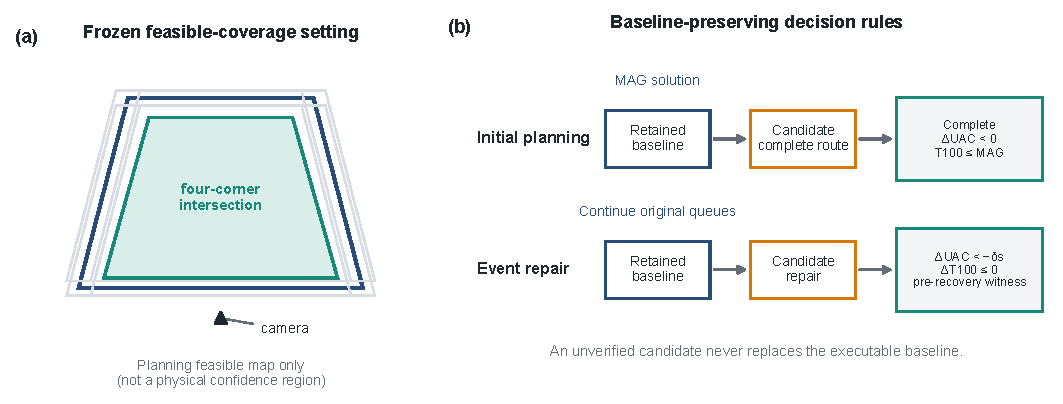
\includegraphics[width=\textwidth]{figure2_baseline_rules.pdf}
\caption{Frozen feasible-coverage setting and baseline-preserving decisions. (a) The implementation uses a four-corner field-of-view intersection as the common planning map; it is not interpreted as a physical confidence region and does not create realized coverage. (b) Initial search retains MAG, whereas event repair retains continuation of the original queues. A candidate replaces its baseline only after the corresponding UAC and T100 checks pass.}\label{fig:baseline-rules}
\end{figure*}

\subsection{Event-Triggered Residual-Task Repair}

A device-unavailable event freezes the confirmed set and marks the device's uncompleted tasks as temporarily unavailable. Tasks currently running on healthy devices and their remaining queues are retained. Let $\mathcal U$ be the set of unconfirmed cells. Among tasks in the unavailable device's original queue, only cells not already covered by the remaining healthy queues form the transferable set $\mathcal X\subseteq\mathcal U$. This rule avoids perturbing healthy work for cells that are already scheduled elsewhere.

The residual timing origin for each healthy device is its predicted pose and conservative remaining duration after the currently active task. Continuing the retained queues defines the executable baseline $\Pi^0$. The repair search inserts viewpoints that can cover $\mathcal X$ into healthy queues, with no more than three accepted insertions and a 40~ms wall-clock budget. Let $\Pi^+$ be a candidate and $\delta_s$ the switching threshold. It is committed only if

\begin{equation}\label{eq:repair-accept}
\overline{\mathrm{UAC}}_H(\Pi^+)
<\overline{\mathrm{UAC}}_H(\Pi^0)-\delta_s,
\qquad
\bar T_{100}(\Pi^+)\leq\bar T_{100}(\Pi^0).
\end{equation}

In addition, at least one transferred cell must have a predicted confirmation time earlier than the unavailable device's earliest recovery time minus margin $\delta_w$. This pre-recovery witness links a queue change to an observable opportunity that could not arise merely by waiting for the original device. The recovery event uses the same baseline comparison before tasks are returned, which avoids oscillation caused by a device briefly reappearing. Planning runs concurrently with the healthy devices' current actions; an event on one device therefore does not impose a team-wide planning pause.

\begin{proposition}[Baseline preservation in event repair]\label{prop:repair}
Every committed repair reduces predicted residual UAC relative to $\Pi^0$ by at least $\delta_s$, does not increase predicted residual T100, and contains a predicted reassigned-coverage witness before recovery.
\end{proposition}

\begin{proof}
The original-queue continuation $\Pi^0$ remains executable while the bounded search evaluates candidates. A candidate replaces it only after Equation~\eqref{eq:repair-accept} and the pre-recovery witness check pass. The stated properties are therefore invariants of the commit operation. They concern the calibrated residual model; whether the witness becomes a confirmed hardware observation is tested from the execution ledger.
\end{proof}

\subsection{Scope of the Formal Properties}

The four propositions occupy different evidential levels. Proposition~\ref{prop:initial} is a planning invariant: it compares two plans under a shared admissible map and time model. Proposition~\ref{prop:evidence} is a log-to-model consistency statement: it connects a coverage write to the measurements required by the implementation. Proposition~\ref{prop:complete} is conditional and makes the reachability and eventual-completion assumptions explicit. Proposition~\ref{prop:repair} is again a planning invariant, now for the residual problem. None alone proves physical superiority over a baseline. Physical superiority requires frozen, paired hardware observations, while physical geometric accuracy would require external calibration evidence not available in the present platform. Keeping these levels separate is essential to the interpretation of the experiments.

